\documentclass[11pt,a4paper]{article}

\usepackage[left=2cm, top=2.5 cm, text={17cm, 24cm}]{geometry}
\usepackage[czech]{babel}
\usepackage[utf8]{inputenc}
\usepackage{times}
\usepackage{amsmath, amsthm, amssymb}
\usepackage{multirow}
\usepackage{multicol}
\usepackage[ruled,czech,linesnumbered,longend,noline]{algorithm2e}
\usepackage{algorithmic}
\usepackage{picture}
\usepackage{graphics}
\usepackage{lscape}
\usepackage{natbib}
\usepackage[IL2]{fontenc}
\usepackage[hidelinks]{hyperref}
\usepackage{breakurl}


\newcommand{\myuv}[1]{\quotedblbase #1\textquotedblleft}

\begin{document}

	\renewcommand{\refname}{}
	\begin{titlepage}
		\begin{center}
			\textsc{\Huge Vysoké učení technické v Brně\\ \medskip
				\huge Fakulta informačních technologií}\\[30mm]

			\begin{center}
				\scalebox{1} {
\includegraphics{fit_logo.eps}}
			\end{center}
			\vspace{\stretch{0.3}}

			\Huge{Implementácia interpretu imperatívneho jazyka}\\[4mm]
			\Huge{IFJ16}\\[2mm]
			\LARGE{Tím 036, variant a/2/II}\\
			\LARGE{Rozšírenia: SIMPLE, BOOLOP}\\

			\vspace{\stretch{0.8}}

			\begin{flushright}
				\noindent \underline{Jakub Semrič}\\
				Petr Rusiňák\\
				Kryštof Rykala\\
				Martin Mikan\\
				\today \hfill         Martin Polakovič \newpage
			\end{flushright}

		\end{center}

		\pagebreak
		\thispagestyle{empty}
		\tableofcontents
		\pagebreak

	\end{titlepage}
	\newpage

	\section{Úvod}

	Tento dokument popisuje návrh a implementáciu interpretu imperatívneho jazyka \emph{IFJ16}, ktorý je podmnožinou jazyka \emph{JAVA SE 8}.
	Program funguje ako konzolová aplikácia, ktorá načíta zdrojový súbor programu v~jazyku IFJ16 a následne ho interpretuje. V~prípade výskytu chyby, program vracia kód chyby.

	Dokument sa skladá z~viacerých častí. V~kapitole \ref{tim} je stručne popísaný vývoj projektu, v~časti \ref{popis} je popísané riešenie jednotlivých častí interpretu, v~kapitole \ref{algoritmy} sa venujeme použitým algoritmom a v~nasledujúcej kapitole \ref{struktury} dátovým štruktúram. Kapitola \ref{rozsirenia} dokumentuje vypracované rozšírenia, kapitola \ref{testovanie} rozoberá náš postup pri testovaní interpretu.


	\section{Práca v tíme}
	\label{tim}

	Keďže sa jednalo o~tímový projekt, na ktorom pracoval tím o~5 členoch, bolo potrebné si určiť opatrenia a~metódy spolupráce. Tie sme si stanovili hneď na začiatku vývojového cyklu. Zaviedli sme konvenciu písania kódu, ktorá nám zabezpečila prehľadnosť a jednotnosť projektu. Taktiež sme zaviedli konvenciu písania komentárov, aby spĺňali normu pre vygenerovanie dokumentácie v nástroji \texttt{doxygen}. K spolupráci viacerých ľudí na jednom projekte sme využili vytvorenie vzdialeného privátneho repozitára na serveri \texttt{GitHub, Inc.}.

	Tímovú komuníkaciu a kolaboráciu sme riešili osobnými stretnutiami, ktoré boli približne raz za tri týždňe. Stanovili sme si ciele, ktoré museli byť do najbližšieho stretnutia dosiahnuté.

	\subsection{Rozdelenie úloh}
	\begin{center}
		\begin{tabular}{|l|l|}
			\hline
			\large{\textbf{Implementovaná časť}} & \large{\textbf{Člen týmu}}\\
			\hline
			\hline
			Lexikálny analyzátor & Kryštof Rykala \\
			\hline
			Parser & Jakub Semrič \\
			\hline
			Precedenčná analýza & Peter Rusiňák \\
			\hline
			Algoritmy, tabuľka symbolov & Martin Polakovič \\
			\hline
			Interpret & Martin Mikan \\
			\hline
		\end{tabular}
	\end{center}

	\subsection{Priebeh vývoja}
	\label{vyvoj}
	Pre nedostatok vedomostí týmu a nestabilitu návrhu, vývoj prebiehal v~niekoľkých
	iteráciach. Na začiatku každej iterácie sa navrhovalo s~primeranou mierou,
	v~ďalšej fáze sa implementovalo a~na konci iterácie sa zamýšľalo ako riešiť
	novo vzniknuté problémy.


	\section{Popis riešenia a implementácia jazyka IFJ16}
	\label{popis}

	Projekt sme implementovali z~niekoľkých funkčných celkov. V nasledujúcich podkapitolách je popis jednotlivých modulov.

	\subsection{Lexikálny analyzátor}
	\label{lexer}
	Lexikálny analyzátor tvorí vstupnú časť interpretu. Model tvorí deterministický
	konečný automat. Spracováva zdrojový súbor a identifikuje v~ňom platné lexémy,
	ktoré posiela syntaktickému analyzátoru vo forme tokenov. Token obsahuje typ lexémy
	a v~prípade aj hodnotu, ak sa jedná o~celočíselný, desatinný alebo reťazcový literál.

	Konečný automat je implementovaný tak, aby vedel spracovať aj jednoduché \texttt{//}
	a~blokové \texttt{/* */} komentáre. Po ukončení komentáru  automat prejde do
	začínajúceho stavu a~začne spracovávať nasledujúcu lexému alebo ďalší komentár.

	Model konečného automatu môžete násjť v~prílohe \ref{app:automat}.


	\subsection{Syntaktický a sémantický analyzátor}
	\label{parser}
	Syntaktický analýzátor (parser) je hlavná časť interpretu. Parser dostáva
	riadenie hneď po otvorení súboru. Má za úlohu nielen preveriť syntax
	a~sémantiku zdrojového súboru, ale taktiež vkladá inštrukcie do inštrukčnej
	pásky. Jeho implementácia spočíva v~rekurzívnom zostupe, ktorý je riadený
	LL gramatikou znázorňenou v~prílohe \ref{gramatika}.

	Keďže jazyk \texttt{IFJ16} je podmnožinou jazyka \texttt{JAVA SE 8},
	ktorého preklad je zložený z dvoch priechodov, je parser zložený
	taktiež z~dvoch priechodov. Prvý priechod analyzuje program zo syntaktického
	a~lexikálneho hľadiska, súčasne vkladá do tabuľky symbolov názvy tried,
	statických funkcií a~premmenných, a kontroluje pokus o redefiníciu.
	Druhý priechod kontroluje semántiku
	programu, spracováva telá funkcií a~vytvára inštrukčnú pásku.



	\subsubsection{Spracovanie jazykových inštrukcií\,--\,rekurzívny zostup}
	\label{rekurzia}
	Rekurzívny zostup riadený LL(1) gramatikou, bol implementovaný tak, že každý
	neterminál v~gramatike bol reprezentovaný funkciou, z~ktorej sa postupne
	volali ďalšie funkcie na základe aktuálneho tokenu a~pravidla v~gramatike.
	Aktuálne načítaný token zase reprezentoval terminálne symboly gramatiky.

	Druhý priechod je taktiež založený na rekurzívnom zostupe, avšak úloha
	jednotlivých funkcií sa od prvého priechodu značne odlišuje.
	Pri inicializácii statických premenných sa výraz za priradením (\texttt{=})
	vyhodnotí precedenčnou analýzou a~vložia sa inštrukcie do hlavného
	inštrukčného listu. Pri analýze funkcií sa postupne vložia ďalšie inštrukcie
	do inštrukčného listu aktuálne spracovávanej funkcie a~v~prípade vyhodnotenia
	výrazu  sa predá riadenie precedenčnej analýze.

	V~prípade volania funkcie sa skontroluje existencia funkcie v~členskej
	triede, počet a~typ parametrov a~v~prípade priradenia  návratový typ
	funkcie a~premennej, do ktorej je volanie priradené. Do inštrukčného
	listu sa vloží inštrukcia \texttt{CALL}, ktorá uloží na hlavný zásobnik
	postupne odkaz na parametre volanej funkcie a~inštrukcia \texttt{LAB}
	iba určí návratový bod, ktorý bude použitý pri skoku z~volanej funkcie.

	Pokiaľ nebola nájdená syntaktická alebo sémantická chyba, po narazení na
	token typu koniec súboru sa v~tabuľke symbolov nájde trieda \emph{Main}
	a~funkcia zapuzdrená v~tejto triede \emph{run()} a~spojí sa hlavný inštrukčný
	list s~inštrukčným listom funkcie \emph{run()}. Pokiaľ požadovane entity
	boli nájdené analýza končí a riadenie je predané interpretu.

	\subsubsection{Precedenčná analýza výrazov}
	\label{precedencna analyza}

	Pre spracovanie výrazov sme použili precedenčnú syntaktickú analýzu zdola nahor,
	riadenú vlastnou gramatikou.
	Parser načítal postupnosť tokenov, ktoré mali byť súčasťou výrazu a predal
	riadenie precedenčnej analýze. Jej výstupom postupnosť inštrukcií, ktoré vyhodnotia tento výraz.

	Precedenčná analýza je implementovaná pomocou precedenčnej tabuľky viz.
	príloha \ref{tabulka} a pomocného zásobníku pre ukladanie výrazov a operátorov.

	Precedenčná tabulka je implementována ako statické pole, kde index prvku je vyjadrený vzťahom $[row * width + col]$.
	Typy tokenov reprezentujúce premenné alebo konštatnty zdieľajú jeden stĺpec.

	Operácie nad zásobníkom sú zjednodušené vynechaním napríklad operácie, ktorá by
	vracala prvok na vrchu zásobníka, keďže táto funkcia nie je potrebná.

	\subsection{Interpret vnútorného kódu}
	\label{interpret}
	Interpret postupne vykonáva inštrukcie v~inštrukčnom liste až kým nenarazí
	na chybu (napr. práca s neinicializovanou premennou) alebo na koniec listu.
	Každá inštrukcia má osobitnú implementáciu. Interpret aktívne využíva hlavný
	zásobník a~zásobník rámcov. Lokálne premenné, s~ktorými má pracovať  sú v~tabuľke,
	ktorá je na vrchole zásobníku rámcov. Statické premenné a~konštanty sú spracovávané
	priamo bez vyhľadania v tabuľke.

	\subsubsection{Volanie a návrat z funkcií}
	\label{funkcia}
	Pri inštrukcii volania funkcie \texttt{CALL} sa podľa prvej adresy
	(3-adresný kód inštrukcie) zistí o~akú funkciu sa jedná a~koľko parametrov
	je na zásobníku. Vytvorí sa nový rámec s lokálnou tabuľkou skopírovanou
	z~lokálnej tabuľky volanej funkcie a súčasne sa naplnia parametre
	hodnotami premenných na zásobníku. Rámec sa uloží na vrchol zásobníku rámcov.
	Nasleduje skok na prvú položku inštrukčného listu danej funkcie.


	Pri inštrukcii \texttt{RET} (príkaz \texttt{return}) nasleduje skok na
	miesto odkiaľ bola funkcia volaná, takže na inštrukciu za inštrukciou
	\texttt{CALL} v predošlom liste. Miesto reprezentované inštrukciou
	\texttt{LAB}\footnote{Label\,--\,inštrukcia reprezentujúca návestie}
	je uložené na hlavný zásobník aby sa vedelo, ktorou inštrukciou
	sa má pokračovať. Návratová hodnota funkcie je uložená v~špeciálnych
	premenných uložených v~globálnej tabuľke symbolov. Jedná sa o emuláciu
	registrov, ktoré zjednodušujú implementáciu celého interpretu.




	\section{Použité algoritmy}
	\label{algoritmy}

	V tejto kapitole pojednávame o popise implementovaný algoritmov potrebným pri tvorbe projektu. Na ich pochopenie a implementáciu bola použitá študijná opora z predmetu IAL (viz prof. \cite{opora}).

	\subsection{Radiaci algoritmus\,--\,Heap Sort}

	Heapsort, radenie haldou, patrí medzi základné algoritmy radenia. Heap\,--\,hromada je
	najčastejšie štruktúra stromového typu, inak tomu nie je ani v našom prípade.
	Pre všetky uzly tohto stromu platí rovnaký vzťah, otcovský uzol je vždy buď
	vačší alebo menší ako jeho synovské uzly. Hromada je implementovaná polom o~veľkosti $N$,
	kde uzol umiestnený na indexe $i$ má svojho ľavého syna na indexe
	$2i+1-base$\footnote{index prvej položky poľa} a~pravého na $2i+2-base$.

	Dôležitou časťou algoritmu je pomocná funkcia \textit{sift down} zabezpečujúca rekonštrukciu hromady. Ak nastane porušenie hromady v koreni, táto funkcia postupnými výmenami dostane prvok z koreňa na správne miesto a do koreňa uloží prvok tak,aby bolo splnené pravidlo hromady. Opakovaným volaním funkcie sift down sa bude v koreni nachádzať prvok s najväčšou hodnotou a tohto faktu potom využívame pri samotnom radení. Odobratý prvok z koreňa sa vždy nahradí najmenším a najpravejším uzlom hromady.

	Táto radiaca metóda má linearitmickú zložitosť.

	\subsection{Vyhľadávací algoritmus\,-- Knuth-Morris-Pratt}

	Jedná sa o algoritmus, využívaný funkciou \textit{find}. Slúži na vyhľadanie vzoru v~reťazci. K~svojej činnosti využíva konečný automat, ktorý je reprezentovaný vektorom prvkov typu \textit{int}, kde index prvku sa zhoduje s~indexom znaku vo vzore a hodnota prvku reprezentuje cieľový index, na ktorý sa má vrátiť pri nezhode porovnania.

	Vyhľadávanie je implementované ako jedna funkcia, ktorej parametrami je ukazovateľ na prehľadávaný reťazec a ukazovateľ na vzor. Na začiatku funkcie sa vytvorí vyššie spomínaný vektor \texttt{fail\_vector}. Následne algoritmus sekvenčne prechádza prehľadávaný reťazec a vzor a porovnáva ich znaky. Pri nezhode sa index vzoru nastaví na hodnotu, ktorej odpovedá hodnota vo vektore na aktuálnom indexe. Porovnávanie prebieha, pokiaľ index reťazca a vzoru nepresiahne	index ich posledných znakov. Návratovou hodnotou je index prvého vyhľadania vzoru v~reťazci. V~prípade neúspechu $-1$.

	Výhodou algoritmu je, že sa nevracia späť v~prehľadávanom reťazci. Nemusí porovnávať už porovnané prvky. Časová zložitosť algoritmu je ${m+n}$.

	\section{Využívané dátové štruktúry}
	\label{struktury}

	\subsection{Tabuľka s rozptýlenými položkami}
	Tabuľka s rozptýlenými položkami je implementovaná ako pole jednosmerne
	viazaných zoznamov symbolov. Symbol obsahuje
	mimo identifikátora aj ukazateľ na členskú triedu. Vyhľadávanie spočíva
	v~nájdení symbolu s~rovnakým identifikátorom
	a súčasne rovnakou členskou triedou. Toto vyhľadávanie zabráňuje kolíziam
	symbolov rovnakých mien v rôznych úrovniach.
	Kedže lokálne premenné nemajú členskú triedu existuje varianta vyhľadávaní v~tabuľke
	iba s jedným kľúčom.

	V interprete sa používaju dva typy tabuliek: lokálna a~globálna. V~globálnej
	tabuľke sú uložené symboly reprezentujúce triedy, funkcie, konštanty, statické
	premenné a~registre. V~lokálnej tabuľke, sú uložené iba lokálne premenné a~parametre
	funkcií, ktoré majú vlastnú tabuľku symbolov.

	\subsection{Zásobník}
	Zásobník je implementovaný ako pole ukazateľov určitej kapacity. Ak je zásobník
	plný dôjde k automatickej realokácii a zvýšeniu kapacity zásobníku.
	V~interprete sa používaju tri zásobníky. Jeden z~nich sa používa na uloženie
	odkazov na miesta skokov a odkazy na parametre funkcií. Druhý zásobník je
	použitý na ukladanie rámcov, ktoré obsahujú lokálnu tabuľku symbolov.
	Posledný zásobník používa analýza výrazov, ktorá si naň ukladá operandy a~operátory.

	\section{Rozšírenia}
	\label{rozsirenia}

	\subsection{SIMPLE}
	Rozšírenie \emph{SIMPLE} umožňuje skrátený zápis konštrukcií cyklov a
	podmienok vynechaním zložených zátvoriek. Keďže by terminálne symboly
	\texttt{\{ \} } moholi byť vynechané, jednalo by sa už o kontextovú gramatiku.
	Tento problém bol vyriešený implementačne bez zmeny
	gramatiky tak, že sa v prípade absencie zložených zátvoriek namiesto volania
	funkcie reprezentujúcej neterminál \texttt{STLIST}, vložila
	funkcia reprezentujúca neterminál \texttt{STAT}, čiže sa namiesto zloženého
	príkazu vykonal jednoduchý príkaz.

	\subsection{BOOLOP}
	Rozšírenie umožňuje poporovať nový dátový typ\,--\,\emph{boolean}. Interpret
	podporuje deklarácie premenných a~funkcií typu boolean. Navyše
	umožnuje vyhodnocovanie zložených podmienok.

	\section{Testovanie}
	\label{testovanie}
	Návrh testov bol založený na metóde ekvivalenčných tried. Testy mali charakter
	regresných testov, takže zmena zdrojových súborov nebola možná ak
	všetky testy neboli úspešné. Testy sa delili do dvoch skupín\,--\,testy
	detekcie chýb a interpretačné testy. Pri testovaní bol použitý program
	\texttt{gcovr} od \cite{COV}, ktorý nám ukázal aké časti interpretu neboli otestované.
	\newpage
	\section{Použité zdroje}
	\bibliography{dokumentace.bib}{}
	\bibliographystyle{czechiso}

	\newpage
	\section{Prílohy}


	\subsection{Konečný automat}
	\label{app:automat}
	\hspace{2cm}
	\begin{center}
		\scalebox{0.7} {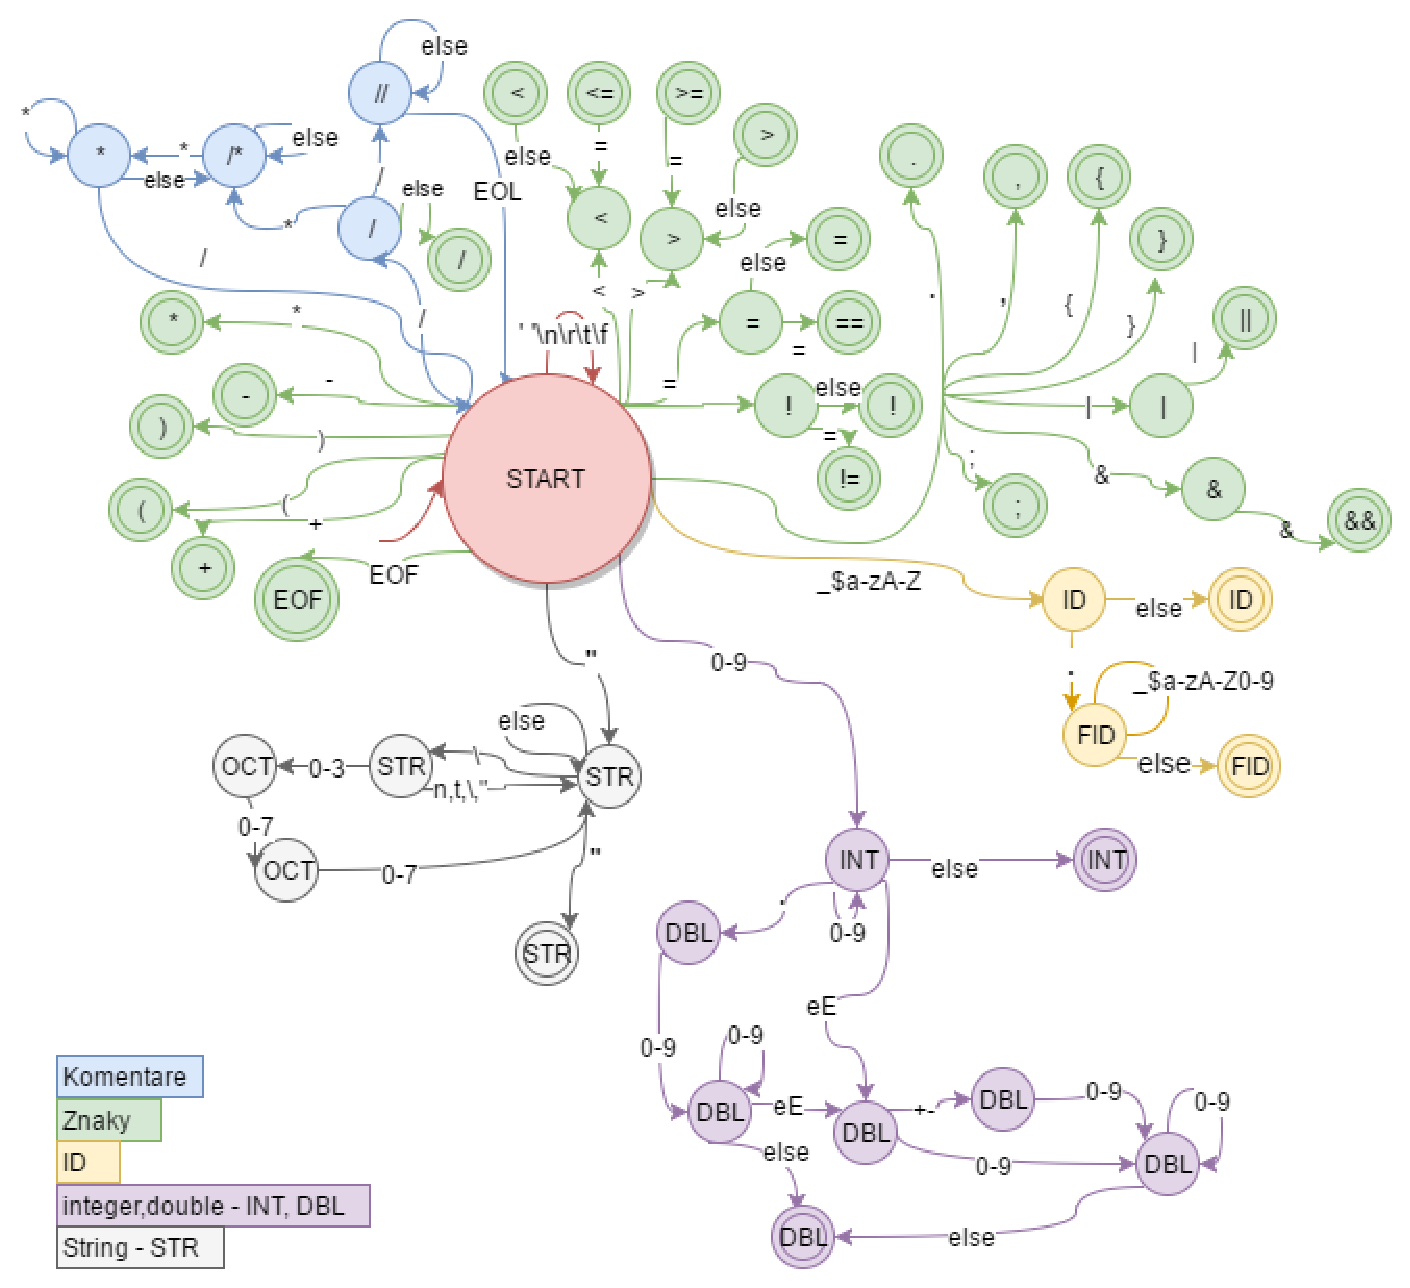
\includegraphics{IFJ.eps}}
	\end{center}


	\newpage

	\subsection{LL(1) gramatika}
	\label{gramatika}
	\begin{tabular}{l c l}
		PROG & $\rightarrow$ & BODY eof \\
		BODY & $\rightarrow$ & CLASS BODY \\
		BODY & $\rightarrow$ & $\epsilon$ \\
		CLASS & $\rightarrow$& class id \{ CBODY \} \\
		CBODY &$\rightarrow$& static TYPE id CBODY2 CBODY \\
		CBODY &$\rightarrow$& $\epsilon$ \\
		CBODY2 &$\rightarrow$& INIT ; \\
		CBODY2 &$\rightarrow$& FUNC \\
		FUNC &$\rightarrow$& ( PAR ) FBODY \\
		FBODY &$\rightarrow$& \{ STLIST \} \\
		PAR &$\rightarrow$& TYPE PAR2 \\
		PAR &$\rightarrow$& $\epsilon$ \\
		PAR2 &$\rightarrow$& $\epsilon$ \\
		PAR2 &$\rightarrow$& id PAR3 \\
		PAR3 &$\rightarrow$& , TYPE id PAR3 \\
		PAR3 &$\rightarrow$& $\epsilon$ \\
		STLIST &$\rightarrow$& STAT STLIST \\
		STLIST &$\rightarrow$&  $\epsilon$ \\
		STAT &$\rightarrow$& while ( EXPR ) \{ STLIST \} \\
		STAT &$\rightarrow$& if ( EXPR ) \{ STLIST \} ELSE \\
		STAT &$\rightarrow$& return RET ; \\
		STAT &$\rightarrow$& id = CALLEXPR ; \\
		STAT &$\rightarrow$& fullid = CALLEXPR ; \\
		STAT &$\rightarrow$& static TYPE id INIT ; \\
		STAT &$\rightarrow$& TYPE id INIT ; \\
		CALLEXPR &$\rightarrow$& fullid ( ARG ) \\
		CALLEXPR &$\rightarrow$& id ( ARG ) \\
		CALLEXPR &$\rightarrow$& EXPR \\
		ARG &$\rightarrow$& $\epsilon$ \\
		ARG &$\rightarrow$& id ARG2 \\
		ARG &$\rightarrow$& fullid ARG2 \\
		ARG2 &$\rightarrow$& $\epsilon$ \\
		ARG2 &$\rightarrow$& , ARG3 ARG2 \\
		ARG3 &$\rightarrow$& fullid \\
		ARG3 &$\rightarrow$& id \\
		INIT &$\rightarrow$& = CALLEXPR \\
		INIT &$\rightarrow$& $\epsilon$ \\
		RET &$\rightarrow$& EXPR \\
		RET &$\rightarrow$& $\epsilon$ \\
		ELSE &$\rightarrow$& $\epsilon$ \\
		ELSE &$\rightarrow$& else ELSE2 \\
		ELSE2 &$\rightarrow$& if ( EXPR ) \{ STLIST \} ELSE \\
		ELSE2 &$\rightarrow$& \{ STLIST \} \\
		TYPE &$\rightarrow$& void \\
		TYPE &$\rightarrow$& int \\
		TYPE &$\rightarrow$& string \\
		TYPE &$\rightarrow$& double \\
		TYPE &$\rightarrow$& boolean \\
	\end{tabular}


	\newpage
	\subsection{Precedenčná tabuľka}
	\label{tabulka}
	\begin{tabular}{|c|c|c|c|c|c|c|c|c|c|c|c|c|c|c|c|c|c|}
		\hline
		& + & - & / & * & ==& !=& \textless & \textgreater & \textless = & \textgreater = & \&\& & \textbar \textbar & ! & ( & ) & i & \$
		\\ \hline
		+  & \textgreater & \textgreater & \textless & \textless & \textgreater & \textgreater & \textgreater & \textgreater & \textgreater & \textgreater & \textgreater & \textgreater & \textless & \textless & \textgreater & \textless & \textgreater
		\\ \hline
		-  & \textgreater & \textgreater & \textless & \textless & \textgreater & \textgreater & \textgreater & \textgreater & \textgreater & \textgreater & \textgreater & \textgreater & \textless & \textless & \textgreater & \textless & \textgreater
		\\ \hline
		/  & \textgreater & \textgreater & \textgreater & \textgreater & \textgreater & \textgreater & \textgreater & \textgreater & \textgreater & \textgreater & \textgreater & \textgreater & \textless & \textless & \textgreater & \textless & \textgreater
		\\ \hline
		*  & \textgreater & \textgreater & \textgreater & \textgreater & \textgreater & \textgreater & \textgreater & \textgreater & \textgreater & \textgreater & \textgreater & \textgreater & \textless & \textless & \textgreater & \textless & \textgreater
		\\ \hline
		== & \textless & \textless & \textless & \textless &   &   & \textless & \textless & \textless & \textless & \textgreater & \textgreater & \textless & \textless & \textgreater & \textless & \textgreater
		\\ \hline
		!= & \textless & \textless & \textless & \textless &   &   & \textless & \textless & \textless & \textless & \textgreater & \textgreater & \textless & \textless & \textgreater & \textless & \textgreater
		\\ \hline
		\textless  & \textless & \textless & \textless & \textless & \textgreater & \textgreater &   &   &   &   & \textgreater & \textgreater & \textless & \textless & \textgreater & \textless & \textgreater
		\\ \hline
		\textgreater  & \textless & \textless & \textless & \textless & \textgreater & \textgreater &   &   &   &   & \textgreater & \textgreater & \textless & \textless & \textgreater & \textless & \textgreater
		\\ \hline
		\textless= & \textless & \textless & \textless & \textless & \textgreater & \textgreater &   &   &   &   & \textgreater & \textgreater & \textless & \textless & \textgreater & \textless & \textgreater
		\\ \hline
		\textgreater= & \textless & \textless & \textless & \textless & \textgreater & \textgreater &   &   &   &   & \textgreater & \textgreater & \textless & \textless & \textgreater & \textless & \textgreater
		\\ \hline
		\&\& & \textless & \textless & \textless & \textless & \textless & \textless & \textless & \textless & \textless & \textless & \textgreater & \textgreater & \textless & \textless & \textgreater & \textless & \textgreater
		\\ \hline
		\textbar \textbar & \textless & \textless & \textless & \textless & \textless & \textless & \textless & \textless & \textless & \textless & \textless & \textgreater & \textless & \textless & \textgreater & \textless & \textgreater
		\\ \hline
		!  & \textgreater & \textgreater & \textgreater & \textgreater & \textgreater & \textgreater & \textgreater & \textgreater & \textgreater & \textgreater & \textgreater & \textgreater & \textless & \textless & \textgreater & \textless & \textgreater
		\\ \hline
		(  & \textless & \textless & \textless & \textless & \textless & \textless & \textless & \textless & \textless & \textless & \textless & \textless & \textless & \textless & = & \textless &
		\\ \hline
		)  & \textgreater & \textgreater & \textgreater & \textgreater & \textgreater & \textgreater & \textgreater & \textgreater & \textgreater & \textgreater & \textgreater & \textgreater & \textgreater &   & \textgreater &   & \textgreater
		\\ \hline
		i  & \textgreater & \textgreater & \textgreater & \textgreater & \textgreater & \textgreater & \textgreater & \textgreater & \textgreater & \textgreater & \textgreater & \textgreater & \textgreater &   & \textgreater &   & \textgreater
		\\ \hline
		\$  & \textless & \textless & \textless & \textless & \textless & \textless & \textless & \textless & \textless & \textless & \textless & \textless & \textless & \textless &   & \textless &
		\\    \hline
	\end{tabular}

\end{document}
